\section{Experiments}\label{Se:Experiments}

We implemented our approach for \ourtask{} in a neural model called \textbf{CPO}, short for Contextual Code Changes via Path Operations.
The main contributions of our approach are (a) the syntactic representation of code edits; and (b) modeling of the likelihood of code edits, rather than modeling the likelihood of the edited code.
Thus, these are the main ideas that we wish to evaluate.
We compare our model with baselines that represent each of the different paradigms (\Cref{Ti:baselines}) on a new dataset. Our model shows significant performance improvement over the baselines. 



\begin{table}[t]
\small
\begin{tabular}{lccc}
\toprule
\multicolumn{1}{l}{} &\multicolumn{1}{l}{\bf Train} &\multicolumn{1}{l}{\bf Validation} &\multicolumn{1}{l}{\bf Test}
\\ 
\midrule
\# projects                                                &38  &8  &7\\
\# examples                                                &39504  &4468  &5934\\
Avg. number of paths                                       &474  &514  &405\\
Avg. number of edit operations                             &2.6  &2.5  &2.7\\
Avg. number of \textbf{\scode{MOV}}                        &36.4\%  &38.3\%  &41.4\%\\
Avg. number of \textbf{\scode{DEL}}                        &48.6\%  &50\%  &50.8\%\\
Avg. number of \textbf{\scode{INS}}                        &5\%  &4.5\%  &2.8\%\\
Avg. number of \textbf{\scode{UPD}}                        &10.1\%  &7.3\%  &5\%\\
Avg. size of moved subtrees (\textbf{\scode{MOV}})         &3.48  &2.95  &2.85\\
Avg. size of deleted subtrees (\textbf{\scode{DEL}})       &4.49  &4.97  &4.39\\
Avg. size of inserted subtrees (\textbf{\scode{INS}})      &1.27  &2.09  &1.26\\
\bottomrule
\end{tabular}
\caption{Statistics over our dataset.}
\label{Ti:dataset_stats}
\end{table} 
\subsection{Dataset}
We introduce a new \ourtask{} dataset of code edits in C\#. We scraped the 53 most popular C\# repositories from GitHub
and extracted all commits since the beginning of the project's history. From each commit, we extracted edits in C\# files along with the edits in their surrounding context. 
Note that a given edit can be part of the edits in the surrounding context () of one example and can be the edit to be predicted  () of another example. In other words, the same edit can have different roles in different examples.
We verified that both examples reside in the same split (i.e., either both examples are in the training set, or both examples are in the test set), without leakage between the sets.

For each edit, we considered a context radius of 10 lines,  above and 10 lines below the edit. 
Representing long sequences is computationally difficult for baselines that use Transformers \cite{NIPS2017_7181} because Transformers have a quadratic time and space complexity. We thus limited the context to 10 lines before and after the edit for these baselines. To make a fair comparison, we limited this in our model as well.
We filtered out examples having more than 50 nodes in the AST of . 
Choosing 50 nodes at most captured the vast majority of examples (81\%). While the technique works for any number of nodes, we picked a limit of 50 to keep the time and cost of experiments reasonable.

To make the task even more challenging, we filtered out examples for which: (a) the edit in  consists of only \textbf{\scode{DEL}} operations; and (b) edits that both  and its context contain only \textbf{\scode{UPD}} operations such that all updates in  are included in the updates of ,
since these usually reflect simple renaming that is easily predicted by modern IDEs.
Following recent work on the adverse effects of code duplication \cite{lopes2017dejavu, allamanis2019adverse}, we split the dataset into training-validation-test \emph{by project}.
This resulted in a dataset containing 39.5K/4.4K/5.9K train/validation/test set examples, respectively. 
We trained all models and baselines on the training set, performed tuning and early-stopping using the validation set, and report final results on the test set.
\Cref{Ti:dataset_stats} shows a summary of the statistics of our dataset.A list of the repositories we used to create our dataset are shown in \Cref{Ap:dataset}. We make our new dataset publicly available at \url{https://github.com/tech-srl/c3po/} .

\subsection{Baselines} \label{baselines}
The two main contributions of our approach that we wish to examine are:
(a) the syntactic representation of code edits; and (b) modeling edit likelihood, rather than modeling code likelihood.
Since we define the new task of \ourtask{}, we picked strong neural baselines and adapted them to this task, to examine the importance of these two main contributions.

\begin{table}[t]
\small
\begin{tabular}{lcc}
\toprule
    & Textual & Syntactic \\
    \midrule
Code Likelihood & \makecell[c]{SequenceR \\ \citep{DBLP:journals/corr/abs-1901-01808}} & \makecell[c]{Path2Tree \\  \cite{aharoni-goldberg-2017-towards}}  \\
\midrule
Edit Likelihood & \makecell[c]{LaserTagger+CRF \\ \cite{malmi2019lasertagger}} & \makecell[c]{\ctc{}PO \\ (this work)} \\
\bottomrule
\end{tabular}
\caption{A high-level taxonomy of our model and the baselines.}
\label{Ti:baselines}
\end{table}

 
\Cref{Ti:baselines} shows a high-level comparison of our model and the baselines. Each model can be classified across two properties: whether it uses a syntactic or textual representation of the edit, and whether it models the \emph{likelihood of the code} or models the \emph{likelihood of the edit}. 
We put significant effort into performing a fair comparison to all baselines, including subtoken splitting as in our model, lowercasing the subtokens, and replacing generated UNK tokens with the tokens that were given the highest attention score.

\textbf{LaserTagger} \cite{malmi2019lasertagger} - is a textual model that models the \emph{edit likelihood}. LaserTagger learns to apply textual edits to a given text. The model follows the framework of \emph{sequence tagging}, i.e., classifying each token in the input sequence. Each input token is classified into one of: \emph{KEEP}, \emph{DELETE} and \emph{SWAP}, where  belongs to a vocabulary of all common phrases obtained from the training set. While LaserTagger leverages edit operations, it does not take advantage of the syntactic structure of the input. 
Since the original implementation of LaserTagger uses a pre-trained BERT NLP model, which cannot be used for code,
we carefully re-implemented a model in their spirit, without BERT. 
We used the same preprocessing scripts and sequence tags as \citet{malmi2019lasertagger}, and encoded the input using either a bidirectional LSTM or a Transformer \cite{NIPS2017_7181} (LaserTagger and LaserTagger, respectively). We further strengthened these models with neural Conditional Random Fields (CRFs) \cite{ma2016end}.
To represent context edits, we employed a sequence alignment algorithm \citep{10.1093/nar/24.14.2730} and extracted the textual edits. We encoded these context edits using 
a bidirectional LSTM
and concatenated the resulting vector to the model's encoded input. 

\textbf{SequenceR} is a re-implementation of \citet{DBLP:journals/corr/abs-1901-01808}.
SequenceR follows the sequence-to-sequence paradigm from Neural Machine Translation (NMT) with attention \citep{DBLP:journals/corr/LuongPM15} and a copy mechanism \cite{DBLP:journals/corr/GuLLL16}. The input is the subtokenized code snippet, along with the textual edits in the context. The output is the edited code. Hence, this method does not take advantage of syntax or edit operations.
We carefully re-implemented this approach because 
SequenceR \emph{abstracts away} identifier names, and replaces identifier names with generic names. For example \scode{int x = 0} becomes \scode{int varInt = 0}. 
Since our model uses identifier names and we found that identifier names help our model, 
to perform a fair comparison -- we kept identifier names in SequenceR as well. 
While the original SequenceR uses LSTMs with copy and attention (SequenceR), our re-implementation allowed us to strengthen this baseline by replacing
the LSTM with a Transformer \cite{NIPS2017_7181} and a copy mechanism (SequenceR). We evaluated both SequenceR, which follows the original model of \citet{DBLP:journals/corr/abs-1901-01808}, and the strengthened SequenceR baseline. 

\textbf{Path2Tree} follows \citet{aharoni-goldberg-2017-towards}. This baseline leverages the syntax and models the code likelihood. In this baseline, we performed a pre-order traversal of the AST and represented the AST as a serialized sequence of nodes. Using this sequential serialization of the AST, we could employ strong neural seq2seq models. The input consists of the paths that represent edits in the context (as in our model), along with a serialized sequence that represents the AST of . The output of the model is the sequence that represents the AST of . 
As the neural underlying seq2seq model, we used both a Transformer (Path2Tree) with a copy mechanism and a BiLSTM with attention and copy mechanisms (Path2Tree) .


\subsection{Setup}
From each sample in our dataset, we (a) extracted all paths of 
 that describe possible valid edit operations; and (b) extracted the paths that represent the transformation of  to , i.e., . We did not filter, discard any of these paths, or limited the paths lengths.

We used input embedding dimensions of 64, LSTM cells with a single layer, and 128 units. This resulted in a very lightweight model of only 750K learnable parameters. 
We trained our model on a Tesla V100 GPU using the Adam optimizer \citep{kingma2014method} with a learning rate of 0.001 to minimize the cross-entropy loss. We applied a dropout \citep{DBLP:journals/corr/abs-1207-0580} of . 


In the baselines, 
we used BiLSTMs with 2 layers having an embedding and hidden state of size 512; this resulted in 10M learned parameters in SequenceR and in Path2Tree resulting in 10M learned parameters. We used the original hyperparameters of the Transformer \citep{NIPS2017_7181} to train Transformers in SequenceR and Path2Tree, resulting in 45M learned parameters. 
LaserTagger uses BiLSTMs with 2 layers having a hidden state size of 128 and an embedding size of 64. This model contained 1M learned parameters. For LaserTagger, we used 4 layers of Transformer encoders, with 4 layers and 8 attention heads, an embedding size of 64, and a hidden state size of 512. For both, the context encoders use BiLSTMs with 2 layers having a hidden state size of 128 and an embedding size of 64. We experimented with LaserTaggers 
that contain a context encoder that uses Transformer and setups
that contained larger dimensions, but they achieved slightly lower results. In the other baselines, larger dimensions contributed positively to the performance.


\paragraph{Evaluation Metric}
To perform a fair comparison across all examined models, we had to use a metric that would be meaningful and measurable in all models and baselines. 
We thus measured exact-match accuracy across all models and baselines.
The accuracy of each model is the percentage of examples in the test set for which
the entire target sequence was predicted correctly. 

\subsection{Results}
\begin{table}[t]
\small
\begin{tabular}{lccc}
\toprule
\multicolumn{1}{l}{\bf Model} &\multicolumn{1}{l}{\bf Acc} & \textbf{Learnable Parameters}  & \textbf{Training Time} 
\\ 
\midrule
SequenceR \citep{DBLP:journals/corr/abs-1901-01808} +copy &30.7 & 10M & 14h\\
SequenceR \citep{DBLP:journals/corr/abs-1901-01808} +copy &32.6  &45M &20h\\
LaserTagger \cite{malmi2019lasertagger} +CRF &40.9 & 1M & 10h\\
LaserTagger \cite{malmi2019lasertagger} +CRF &41.4 &1.6M & 20h\\
Path2Tree \cite{aharoni-goldberg-2017-towards} +copy &22.5 & 10M & 24h\\
Path2Tree \cite{aharoni-goldberg-2017-towards} +copy &25.6  & 45M & 24h\\
\midrule
\ctc{}PO (this work)  &\textbf{53.2} & \textbf{750K}  & \textbf{9h}\\
\bottomrule

\end{tabular}
\caption{Our model achieves significantly higher accuracy than the baselines.}
\label{Ti:results}
\end{table}

 
\paragraph{Performance}
\Cref{Ti:results} depicts the main results of our evaluation: \ctc{}PO gains more than 11\% absolute accuracy over LaserTagger, which performed the best of all baselines. 
These results emphasize the need for structural representation of both edits and context. \ctc{}PO achieves accuracy that is twice that of the syntactic baseline Path2Tree. Although this baseline uses AST paths to represent the changes in the context of  and to represent  with its underlying AST, its performance is inferior compared to our \ctc{}PO. This is because Path2Tree does not model the edit operations directly and thus needs to generate the entire AST of . 


These results show the significance of our model’s two main contributions. \emph{Modeling the edit} has the most significant contribution as expressed in the advantage of our model over both versions of Path2Tree, and in the advantage of both versions of LaserTagger over both versions of SequenceR.
Syntactic representation over textual representation also has a significant contribution, which is expressed in the superiority of our model over both versions of LaserTagger.
Using these two key contributions, our model performs significantly better than all models, while being much more lightweight in terms of learnable parameters. The same results are visualized in \Cref{csharp_results_barchart_figure}.

\definecolor{sequencerlstm}{HTML}{0F9D58}
\definecolor{sequencertrans}{HTML}{000080}
\definecolor{lazerlstm}{HTML}{FF6d00}
\definecolor{lazertrans}{HTML}{46BDC6}
\definecolor{path2treelstm}{HTML}{4285F4}
\definecolor{path2treetrans}{HTML}{DB4437}
\definecolor{ccc}{HTML}{AB30C4}

\begin{figure}[h]
\centering
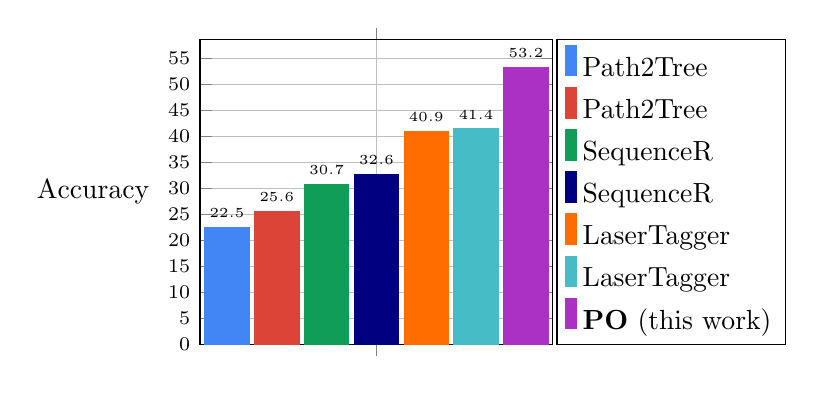
\begin{tikzpicture}
\begin{axis}[
    ybar,
    bar width=16pt,
    width=0.5\textwidth,
    height=5.45cm,
    enlarge x limits=0.10,
    ylabel={Accuracy},
    symbolic x coords={\ },
    xtick=data,
    x tick label style  = {font=\normalsize},
    nodes near coords style={
        color=black,
        font=\tiny
    },nodes near coords,
    font=\scriptsize,
    legend style={font=\normalsize,at={(1.01,0.5)},
    legend cell align={left},
    anchor=west, row sep=0.5pt},
    legend image code/.code={\draw[#1, draw=none] (0cm,-0.1cm) rectangle (0.15cm,0.3cm);
            },
    ytick={0.0,5.0,...,60.0},
    ymin=0,
    grid = major,
    grid style={line width=0.1pt, draw=gray!10},
    major grid style={line width=.2pt,draw=gray!50},
    ylabel style={rotate=-90,font=\normalsize},
    ]
\addplot[path2treelstm,fill=path2treelstm] coordinates {(\ ,22.5)};
\addplot[path2treetrans,fill=path2treetrans] coordinates {(\ ,25.6)};
\addplot[sequencerlstm,fill=sequencerlstm] coordinates {(\ ,30.7)};
\addplot[sequencertrans,fill=sequencertrans] coordinates {(\ ,32.6)};
\addplot[lazerlstm,fill=lazerlstm] coordinates {(\ ,40.9)};
\addplot[lazertrans,fill=lazertrans] coordinates {(\ ,41.4)};
\addplot[ccc,fill=ccc] coordinates {(\ ,53.2)};
\legend{
    Path2Tree,
    Path2Tree,
    SequenceR,
    SequenceR,
    LaserTagger,
    LaserTagger,
    \textbf{\ctc{}PO} (this work)
}
\end{axis}
\end{tikzpicture}
\caption{Visualization of the accuracy score of our model compared to the baselines. The values are the same as in \Cref{Ti:results}. Our model achieves significantly higher
accuracy than the baselines.}
\label{csharp_results_barchart_figure}
\end{figure}  \definecolor{c3pocolor}{HTML}{AB30C4}



\begin{figure}[t]
\centering
\begin{tikzpicture}[scale=1, trim left=-1.5cm]
	\begin{axis}[
		xlabel={Context radius (lines)},
		ylabel={\footnotesize{Acc}},
		ylabel near ticks,
        xmin=0, xmax=11,
        ymin=-5, ymax=100,
        xtick={1,2,3,4,5,6,7,8,9,10},
        xticklabels={1,2,3,4,5,6,7,8,9,10},
        ytick={0,10,...,100},
        label style={font=\footnotesize},
        ylabel style={rotate=-90,font=\scriptsize},
        ylabel style={font=\scriptsize},
        xlabel style={font=\footnotesize},
        tick label style={font=\scriptsize} ,
        grid = major,
        major grid style={dotted,black},
        width = 0.8\linewidth, height = 5cm,
        name = first
    ]
    \addplot[color=c3pocolor,mark options={fill=c3pocolor, draw=black, line width=0.5pt}, line width=1pt, mark=*, mark size=2pt] coordinates {
    (1,26.7)
    (2,40)
    (3,45.7)
    (4,56)
    (5,56)
    (6,55.9)
    (7,57.6)
    (8,50.8)
    (9,59)
    (10,50.8)
	};
	\end{axis}
	
		\begin{axis}[
xlabel={Context radius (lines)},
		bar width=16,
		symbolic x coords={0,1,2,3,4,5,6,7,8,9,10,11},
		ylabel={\footnotesize{\# Examples}},
		ylabel near ticks,
        xmin=0, xmax=11,
        xtick=data,
        ytick={0,250,500,...,1750},
        ymin=0,
        ymax=2000,
        label style={font=\footnotesize},
        ylabel style={rotate=-90,font=\scriptsize},
        ylabel style={font=\scriptsize},
        xlabel style={font=\footnotesize},
        tick label style={font=\scriptsize} ,
        grid = major,
        major grid style={dotted,black},
        width = 0.8\linewidth, height = 5cm,
        name=second,
        at=(first.below south west),
        anchor=north west
    ]
        \addplot[ybar,fill=c3pocolor] coordinates { 
        (1,30)
        (2,252)
        (3,212)
        (4,353)
        (5,412)
        (6,602)
        (7,571)
        (8,931)
        (9,884)
        (10,1684)
        };
	\end{axis}

\end{tikzpicture}
\caption{The upper figure depicts the accuracy as a function of the context radius size. The lower figure shows the number of examples per radius size in the test set.}
\label{acc-by-ctx-radius}
\end{figure}  
\paragraph{Path2Tree Lower Performance Compared to SequenceR}
Although Path2Tree represents the edits syntactically (which we believe to be a better representation, in general) and SequenceR represents edits textually, the results of Path2Tree are lower than those of SequenceR.

We believe that the main limitation of Path2Tree is that it cannot easily generalize between the program fragment  and the given context . This occurs because  is represented as paths, while  is generated as a tree. In contrast, SequenceR represents all inputs and outputs the same, i.e., as sequences of tokens. We also performed initial experiments with a Tree2Tree baseline that encodes , , and  as trees and generates  as a tree, thus potentially having a better generalization ability than Path2Tree. However, Tree2Tree achieved much lower results than Path2Tree, because the tree encoding created very large inputs, especially in . These, prevented the model from properly capturing the edits that occurred in the context (), while the encoding of  as paths is much more succinct and focused (and performed better than Tree2Tree).


\subsection{Scalability Analysis}
We conducted an analysis of our model that shows the performance of \ctc{}PO as a function of the context radius size and the number of nodes.

\Cref{acc-by-ctx-radius} shows the accuracy of \ctc{}PO compared to the context radius size, i.e., the number of lines between the beginning of  and .
As shown, the accuracy of \ctc{}PO remains stable when the context radius increases. This hints that the context radius can be further increased without sacrificing accuracy. In our experiments, we put this limitation only to limit the size of the dataset.



\Cref{acc-by-num-nodes} shows the accuracy of \ctc{}PO compared to the number of nodes in the AST of . As the size of  increases, our model shows a natural descent, and the accuracy stabilizes for sizes of 31 nodes and above. As shown in the lower part of \Cref{acc-by-num-nodes}, the number of examples also decreases with the size of the edit: the most common edits have 11 to 15 nodes, in which our model achieves an accuracy of 80\%.












\definecolor{c3pocolor}{HTML}{AB30C4}

\begin{figure}[t]
\centering
\begin{tikzpicture}[scale=1, trim left=-1.5cm]
	\begin{axis}[
		xlabel={\# nodes},
		ylabel={\footnotesize{Acc}},
		ylabel near ticks,
        xmin=0, xmax=55,
        ymin=-5, ymax=105,
         xtick={5,10,15,20,25,30,35,40,45,50},
        xticklabels={0--5,6--10,11--15,16--20,21--25,26--30,31--35,36--40,41--45,46--50},
        ytick={0,10,...,100},
        label style={font=\footnotesize},
        ylabel style={rotate=-90,font=\scriptsize},
        ylabel style={font=\scriptsize},
        xlabel style={font=\footnotesize},
        tick label style={font=\scriptsize} ,
        grid = major,
        major grid style={dotted,black},
        width = 0.8\linewidth, height = 5cm,
        name = first
    ]
    \addplot[color=c3pocolor,mark options={fill=c3pocolor, draw=black, line width=0.5pt}, line width=1pt, mark=*, mark size=2pt] coordinates {
    (5,100)
    (10,88.9)
    (15,79.6)
    (20,55.8)
    (25,35.8)
    (30,34.3)
    (35,21)
    (40,22.5)
    (45,21.7)
    (50,22.4)
	};
	\end{axis}
	
		\begin{axis}[
xlabel={\# nodes},
		bar width=16,
		symbolic x coords={0, 0--5,6--10,11--15,16--20,21--25,26--30,31--35,36--40,41--45,46--50, 55},
		ylabel={\footnotesize{\# Examples}},
		ylabel near ticks,
        ytick={0,250,500,...,1500},
        ymin=0,
        ymax=1750,
        label style={font=\footnotesize},
        ylabel style={rotate=-90,font=\scriptsize},
        ylabel style={font=\scriptsize},
        xlabel style={font=\footnotesize},
        tick label style={font=\scriptsize} ,
        grid = major,
        major grid style={dotted,black},
        width = 0.8\linewidth, height = 5cm,
        name=second,
        at=(first.below south west), 
        anchor=north west
    ]
        \addplot[ybar,fill=c3pocolor] coordinates { 
        (0--5,10)
        (6--10,718)
        (11--15,1498)
        (16--20,919)
        (21--25,772)
        (26--30,655)
        (31--35,496)
        (36--40,462)
        (41--45,267)
        (46--50,138)
        };
	\end{axis}

\end{tikzpicture}
\caption{The upper figure depicts the accuracy as a function of the number of nodes in . The lower figure shows the number of examples compared to the number of nodes in .}
\label{acc-by-num-nodes}
\end{figure}  

\subsection{Qualitative Analysis}
We manually examined the predicted examples and discuss two representative cases.

\Cref{Fi:qa_mov_exmp} shows an example in which the modification of a method signature in the context affects , which lies in the method body.
The context of , shown in \Cref{Fi:qa_mov_exmp_a}, includes a change in the signature of the method \scode{GetFileCharacteristic}. 
The name of the method was changed to \scode{GetAppender} and its return type was updated from \scode{FileCharacteristic} to \scode{BaseFileAppender}.

Consider  in \Cref{Fi:qa_mov_exmp_b}.  is a return statement, located in the body of the changed method \scode{GetFileCharacteristic}. Since the return type of the method was updated to \scode{BaseFileAppender}, the return statements inside the method must be changed as well.  The renaming of the method to \scode{GetAppender} may have also hinted to our model that the \scode{appender} object itself should be returned.
Our model successfully predicted the desirable edit, altering the return statement from \scode{return appender.GetFileCharacteristic} to \scode{return appender;}. 
This example shows how context edits are important in predicting edits in a program, 
by providing information about (a) return type changes and (b) method renaming.

\begin{figure}[t]
\begin{subfigure}[b]{.49\textwidth}
  \centering
  \includegraphics[scale=0.45]{figures/mov_exmp_a.pdf}  
  \caption{}
  \label{Fi:qa_mov_exmp_a}
\end{subfigure}
\begin{subfigure}[b]{.49\textwidth}
  \centering
  \includegraphics[scale=0.45]{figures/mov_exmp_b.pdf}  
  \caption{}
  \label{Fi:qa_mov_exmp_b}
\end{subfigure}
\caption{
An example where the edit of a method signature affects the edit of  which lies in the method body. \Cref{Fi:qa_mov_exmp_a} illustrates the edit in the context and the paths that describe the transformation from  to . \Cref{Fi:qa_mov_exmp_b} shows the predicted edit operations along with their associated paths in .}
\label{Fi:qa_mov_exmp}
\end{figure} 
\Cref{Fi:qa_ins_exmp} illustrates a case where the edit in the context is conceptually similar to the edit in , but is not identical. 
\Cref{Fi:qa_ins_exmp_a} shows a variable declaration statement, where \scode{part} is cast to the type \scode{MethodCallExpression} and assigned to the newly-declared variable \scode{methodExpression}. In the edited context, the keyword \scode{var} was updated to an explicit type \scode{MethodCallExpression}. 
\Cref{Fi:qa_ins_exmp_b} shows an edit that is similar in spirit:  consists of an initialization statement, where the variable \scode{nameParts} is  assigned a new \scode{Stack<string>}. Using the edit in the context, our model predicted the edit of \scode{var} to \scode{Stack<string>} in . This edit consists of an insertion of a new subtree, since \scode{Stack<string>} is represented as a subtree of five nodes. In contrast, the edit in the context is represented as an \textbf{\scode{UPD}} edit, because it only needs to update the value of a single node. 
This example demonstrates a class of examples where the edit in the context hints edits that are similar in spirit in , but are not identical and should be performed differently.

\begin{figure}[t]
\begin{subfigure}[b]{.49\textwidth}
  \centering
  \includegraphics[scale=0.45]{figures/ins_exmp_a.pdf}  
  \caption{}
  \label{Fi:qa_ins_exmp_a}
\end{subfigure}
\begin{subfigure}[b]{.49\textwidth}
  \centering
  \includegraphics[scale=0.45]{figures/ins_exmp_b.pdf}  
  \caption{}
  \label{Fi:qa_ins_exmp_b}
\end{subfigure}
\caption{
An example in which the edit in the context is conceptually similar to the edit of . \Cref{Fi:qa_ins_exmp_a} illustrates the edit that occurred in the context and the paths that describe the transformation from  to . \Cref{Fi:qa_ins_exmp_b} shows the predicted edit operations along with their associated paths in .}
\label{Fi:qa_ins_exmp}
\end{figure} 


